\section{Vergleichbare Arbeiten}
\label{sec02:vergleichbare_arbeiten}
In diesem Abschnitt werden kurz einige Programme beschrieben, die mit grafischer Oberfläche erlauben Datenbanken zu verwalten. Dabei sind keine davon an Anfänger gerichtet, um sich in das Thema der Datenbanken einzuarbeiten. 

%%%%%%%%%%%%%%%%%%%%%%
\subsection{DB SQLite Browser}
\label{sec02:sqlite_browser}
Die von Sqlitebrowser\footnote{\url{http://sqlitebrowser.org/}} entwickelte Open-Source Software soll nicht nur als ein Front-End für das Kommandozeilen Programm dienen. Die Entwickler beschreiben Ihre Software folgendermaßen:
\begin{quote}
``This program is not a visual shell for the sqlite command line tool. It does not require familiarity with SQL commands. It is a tool to be used both by developers and by end users, and it must remain as simple to use as possible in order to achieve its goals.''~\cite{db_sqlite_browser}
\end{quote}

Es soll bedient werden können ohne Kennt­nis von SQL vorauszusetzen. Die einzelnen Befehle werden durch die GUI gesteuert. Dabei werden die einzelnen korrespondierenden SQL-Befele in der Seitenleiste angezeigt.
Der ``DB SQLite Browser'' ist einer der wenigen Programme, die die Migration von SQLite Datenbanken unterstützt. Dabei wird ein Algorithmus, der auf der SQLite Website zu finden ist, verwendet. Dieser wird in der weiteren Arbeit besprochen(siehe Kapitel:~\ref{subsubsec04:sql_vs_ruby}), da dieser Algorithmus einen wichtigen Stellenwert annimmt.

Im DB SQLite Browser ist nicht an Beginner gerichtet. Viele Funktionen werden mit der Benutzeroberfläche bedient. Dabei wird jede Aktion zusätzlich als SQL-Statement angezeigt, was für Beginner eine Hilfe sein kann, oder zur Verwirrung führen kann. 
Fehler werden abgefangen und automatisch behoben. Sollte eine Tabelle mit ``Without RowId'' erstellt werden und kein Primärschlüssel gesetzt werden, wird dieser automatisch hinzugefügt, anstelle einer Fehlermeldung anzuzeigen.
Foreign Keys werden nicht direkt angezeigt, sie sind nur in dem SQL-Create-Statement der Tabellen zu sehen.

\begin{figure}[ht]
    \frame{\includegraphics[width=\textwidth]{images/kap-2-sqlitebrowser.png}}
        \centering
        \caption{DB SQLite Browser}
        \label{pic:sqlite_browser}
\end{figure}


%%%%%%%%%%%%%%%%%%%%%%
\subsection{MySQL Workbench}
\label{sec02:mysql_workbench}
Die MySQL Workbench\footnote{\url{https://www.mysql.de/products/workbench/}} ist ein Datenbank-Modellierungswerkzeug, welches von den Oracle Corporation, den Entwicklern des Datenbanksystems MySQL, entwickelt wurde.
Mit der MySQL Workbench ist es möglich MySQL Datenbanken zu verwalten. Die Software ist an Benutzer mit Grundwissen bis hin zu professionelle Benutzer gerichtet. Es stellt alle Funktionen des Datenbanksystems in einer grafischen Anwendung zur Verfügung. Es lassen sich komplette neue Datenbanken, Insert-Statements und Migrationen grafisch erstellen.

Mit MySQL Workbench lassen sich grafisch Schemata erstellen. Dabei ist es möglich direkt Einträge in die Tabelle einzutragen. Bei der Verwendung der grafischen Erstellung von Schemata, muss MySQL Workbench nicht mit einem Datenbankserver verbunden sein. Die Einträge werden somit nicht validiert. Es gibt zwei Arten von Foreign Keys die in der MySQL Workbench per Knopfdruck erstellt werden können. Zur Visuallisierung werden die Foreign Key Referenzen mit Strichen zwischen den Tabellen dargestellt. Studenten die diese Software im Einführungskurs Datenbanken verwenden, gehen von aus, dass die Workbench die Foreign Keys schon richtig setzt. Dabei erstellt die MySQL Workbench ``Identifying relationships'', was gegebenenfalls nicht vom Benutzer gewollt wird.
MySQL Workbench ist eine sehr funktionsreiche Software, die von Anfängern genutzt werden kann, aber an vielen Stellen, durch mangelndes Wissen, zu Fehlern führen kann. 
\begin{figure}[ht]
    \frame{\includegraphics[width=\textwidth]{images/kap-2-mysql.png}}
        \centering
        \caption{MySQL Workbench}
        \label{pic:mysql_workbench}
\end{figure}

%%%%%%%%%%%%%%%%%%%%%%
\subsection{SQLite Manager}
\label{sec02:sqlite_manager}
Dieses als Plugin bereitstehende DBMS\footnote{\url{https://github.com/lazierthanthou/sqlite-manager}}, für den Firefox, Thunderbird, Komodo u.a. wurde von ``lazierthanthou''\footnote{\url{https://github.com/lazierthanthou}} entwickelt. Als Plugin soll diese Software besonders ressourcensparend sein, und somit bietet es nur die nötigsten Funktionen zum Verwenden einer SQLite Datenbank. Viele Funktionen werden als SQL-Befehle erwartet, welche Schablonenweise aus einem Drop-Down-Menu erstellt werden können.
Dabei werden Migrationen nicht direkt unterstützt und müssen gegebenenfalls selbst erstellt werden.

Damit ist der SQLite Manager als eine schnelle Alternative zu einer Kommandozeilen Konsole. Durch die Auswahl von SQL-Befehle durch ein Drop-Down-Menu bietet es eine Hilfestellung für Benutzer, die die SQL-Befehle noch nicht verinnerlicht haben. Damit ist es keine Software die nur für erfahrene Benutzer bestimmt ist, es ist aber auch keine für Anfänger.
\begin{figure}[ht]
    \frame{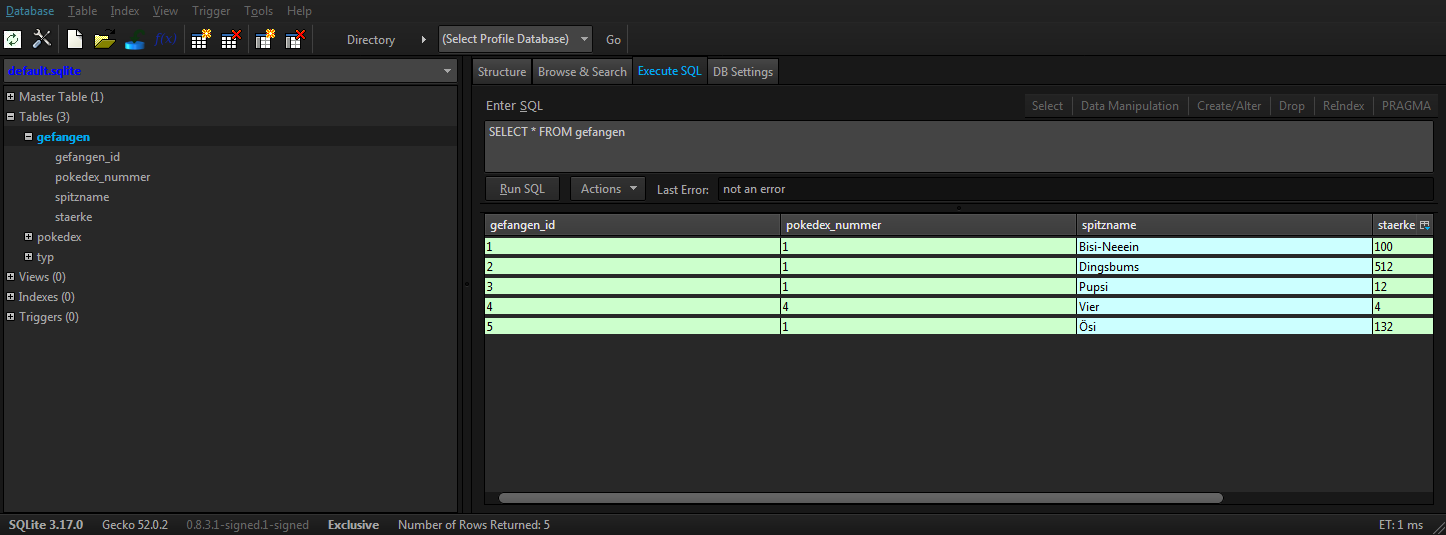
\includegraphics[width=\textwidth]{images/kap-2-sqlitemanager.PNG}}
        \centering
        \caption{SQLite Manager}
        \label{pic:sqlite_manager}
\end{figure}

%%%%%%%%%%%%%%%%%%%%%%
\subsection{Heidi SQL}
\label{sec02:heidi_sql}
Die Software\footnote{\url{https://www.heidisql.com/}} vom deutschen Programmierer ``Ansgar Becker'' wurde ursprünglich als MySQL-Front entwickelt. Es sollte als grafische Bedienoberfläche für MySQL Datenbanken dienen. Es unterstützt alle Funktionen die MySQL bietet. Nachdem das Projekt zu Open-Source wurde, wuchs die Gruppe an Entwicklern. In späteren Versionen wurden weitere Datenbanken unterstützt, wie Microsoft SQL Server und PostgreSQL.
Die Bedienung findet über die grafische Oberfläche statt, somit müssen SQL-Befehle nicht direkt selbst geschrieben werden. Die SQL-Befehle die bei der Bedienung entstehen, werden zusätzlich angezeigt.  

Heidi SQL ist eine funktionsreiche Software. Anfänger können ähnlich wie bei der MySQL Workbench mit der großen Anzahl an Funktionen überfordert sein. Nach einer gewissen Einarbeitungszeit können aber auch Anfänger mit dieser Software, Datenbanken erstellen und bearbeiten. Durch Symbole und Icons werden viele Eigenschaften von Tabellen, so zum Beispiel die Foreign Keys, verständlich und übersichtlich dargestellt. Somit ist die Darstellung und Bedienung für Anfänger geeignet, lediglich die Fülle an Funktionen können dabei hinderlich sein. 
\begin{figure}[ht]
    \frame{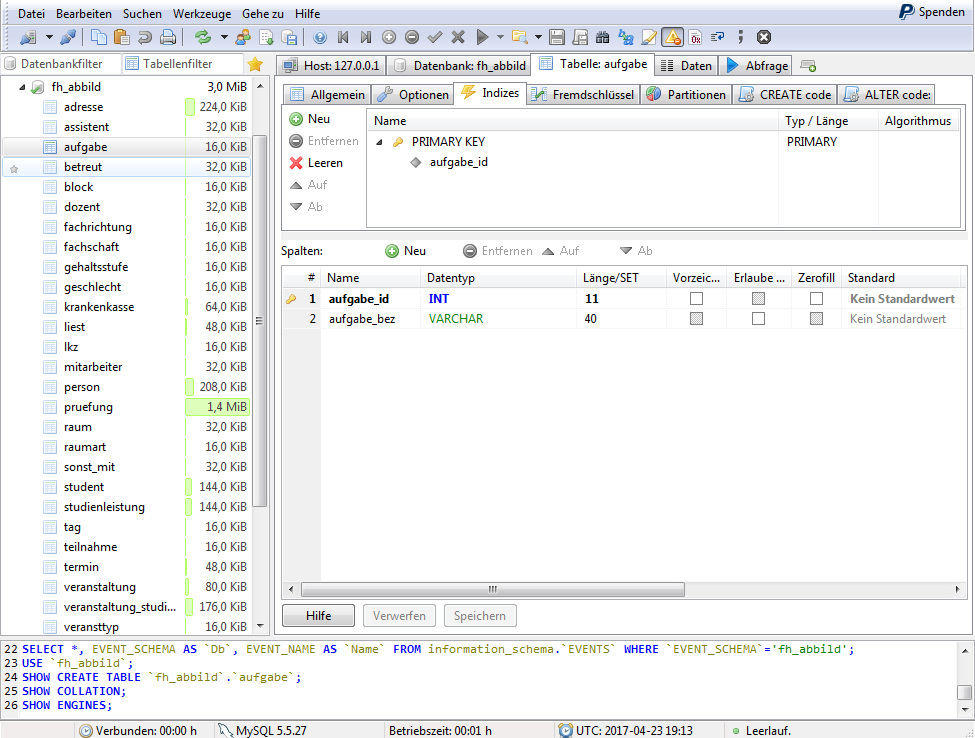
\includegraphics[width=\textwidth]{images/kap-2-heidi.PNG}}
        \centering
        \caption{Heidi SQL}
        \label{pic:heidi_sql}
\end{figure}

%%%%%%%%%%%%%%%%%%%%%%
\subsection{PHP-MyAdmin}
\label{sec02:php_myadmin}
PHP-MyAdmin\footnote{\url{https://www.phpmyadmin.net/}} ist eine webbasierte Anwendung, zur Verwaltung von MySQL Datenbanken. Die Software ist komplett in PHP geschrieben, was zu dem Namen der Anwendung führte. Die Software wurde von Tobias Ratschiller entwickelt, ab 2000 wurde das Projekt von The phpMyAdmin Project weiter entwickelt.
Die Software ist in mehreren Sprachen zur Verfügung gestellt und weit verbreitet. Viele Webhosting Provider verwenden PHP-MyAdmin. Neben der PHP-MyAdmin Anwendung gibt es verwandte Software für die Unterstützung von SQLite Datenbanken.

PHP-MyAdmin ist an sehr erfahrene Benutzer gerichtet. Die Bedienung erfordert keine direkte Eingabe von SQL-Befehlen, jedoch sind die benötigten Informationen die während der Bedienung von PHP-MyAdmin von einem Anfänger nicht zu erwarten.
\begin{figure}[ht]
    \frame{\includegraphics[width=\textwidth]{images/kap-2-phpmyadmin.png}}
        \centering
        \caption{PHP-MyAdmin}
        \label{pic:php_myadmin}
\end{figure}


\subsection{PhpLiteAdmin}
\label{sec02:phpliteadmin} 
PhpLiteAdmin\footnote{\url{https://www.phpliteadmin.org/}} ist eine in PHP geschriebene Software, die die Verwaltung von SQLite Datenbanken unterstützen soll. Die Anwendung soll zusätzlich zu den Funktionen von SQLite selbst, auch unter anderem Migration von Datenbanken unterstützen. Dabei sollen Tabellen und Spalten verändert werden können. 
In der aktuellen Version zur Zeit der Entwicklung dieser Arbeit, führt jede Migration zu einem Fehler. Das Vorgehen zum Verändern einer Tabelle unterscheidet sich deutlich von der SQLite vorgestellten Methode, die auch von DB SQLite Browser~\ref{sec02:sqlite_browser} verwendet wird. 
\begin{itemize}
    \item Es wird eine temporäre Tabelle erstellt in denen alle Datensätze gespeichert werden
    \item Tabelle löschen
    \item Neue Tabelle erstellen nach den Kriterien der Änderungen
    \item Datensätze aus der temporären Tabelle kopieren
    \item Temporäre Tabelle löschen
\end{itemize}
Mit dieser Lösung wird die Funktion von SQLite eine Tabelle umzubennen nicht verwendet. 
Dadurch müssen Foreign Keys zusätzlich bearbeitet werden, wenn der Tabellenname sich verändert hat.

\begin{figure}[ht]
    \frame{\includegraphics[width=\textwidth]{images/kap-2-phpliteadmin.png}}
        \centering
        \caption{PhpLiteAdmin}
        \label{pic:phpliteAdmin}
\end{figure}